% interacttfqsample.tex
% v1.05 - August 2017

\documentclass[]{interact}

\usepackage{epstopdf}% To incorporate .eps illustrations using PDFLaTeX, etc.
\usepackage[caption=false]{subfig}% Support for small, `sub' figures and tables
%\usepackage[nolists,tablesfirst]{endfloat}% To `separate' figures and tables from text if required

%\usepackage[doublespacing]{setspace}% To produce a `double spaced' document if required
%\setlength\parindent{24pt}% To increase paragraph indentation when line spacing is doubled
%\setlength\bibindent{2em}% To increase hanging indent in bibliography when line spacing is doubled

\usepackage[numbers,sort&compress]{natbib}% Citation support using natbib.sty
\bibpunct[, ]{[}{]}{,}{n}{,}{,}% Citation support using natbib.sty
\renewcommand\bibfont{\fontsize{10}{12}\selectfont}% Bibliography support using natbib.sty

\theoremstyle{plain}% Theorem-like structures provided by amsthm.sty
\newtheorem{theorem}{Theorem}[section]
\newtheorem{lemma}[theorem]{Lemma}
\newtheorem{corollary}[theorem]{Corollary}
\newtheorem{proposition}[theorem]{Proposition}

\theoremstyle{definition}
\newtheorem{definition}[theorem]{Definition}
\newtheorem{example}[theorem]{Example}

\theoremstyle{remark}
\newtheorem{remark}{Remark}
\newtheorem{notation}{Notation}

\usepackage{color}
\usepackage{listings}
%% listings-modelica.cfg
%% Copyright 2014 Martin Sjoelund, Dietmar Winkler
%
% This work may be distributed and/or modified under the
% conditions of the LaTeX Project Public License, either version 1.3
% of this license or (at your option) any later version.
% The latest version of this license is in
%   http://www.latex-project.org/lppl.txt
% and version 1.3 or later is part of all distributions of LaTeX
% version 2005/12/01 or later.
%
% This work has the LPPL maintenance status `maintained'.
%
% The Current Maintainer of this work is Dietmar Winkler
%
% Code repository https://github.com/modelica-tools/listings-modelica
%
% This work consists of the file listings-modelica.cfg

\lstdefinelanguage{modelica}
{
  morekeywords=[1]{
    algorithm,and,annotation,as,assert,block,break,case,class,connect,connector,
    constant,constrainedby,der,discrete,each,else,elseif,elsewhen,encapsulated,
    end,enumeration,equality,equation,expandable,extends,external,failure,final,
    flow,for,function,guard,if,import,in,initial,inner,input,List,local,loop,
    match,matchcontinue,model,not,operator,Option,or,outer,output,package,parameter,
    partial,protected,public,record,redeclare,replaceable,return,stream,
    subtypeof,then,Tuple,type,uniontype,when,while},
  morekeywords=[2]{true, false},
  % Do not make true,false keywords because fn(true,x, false ) shows up as fn(true,x, *false*)
  morekeywords=[3]{optimization,constraint}, % Optimica keywords
  morekeywords=[4]{objective,startTime,finalTime,initialGuess},
  sensitive=true,
  comment=[l]//,
  morecomment=[s]{/*}{*/},
  alsodigit={.,-},
  morestring=[b]',
  morestring=[b]",
}[keywords,comments,strings]

\definecolor{keywordcolor1}{rgb}{0,0,.4}
\definecolor{keywordcolor2}{rgb}{.90,0,0}
\definecolor{keywordcolor3}{rgb}{.4,0,.8}
\definecolor{keywordcolor4}{rgb}{0.5,0,0.5}
\definecolor{stringcolor}{rgb}{0.133,0.545,0.133}
% \definecolor{listingbgcolor}{rgb}{0.95,0.95,0.95}

\lstset{
  breaklines=true,
  language=modelica,
  basicstyle=\ttfamily,
  keywordstyle=[1]\color{keywordcolor1}\bfseries,
  keywordstyle=[2]\color{keywordcolor2},
  keywordstyle=[3]\color{keywordcolor3}\bfseries,
  keywordstyle=[4]\color{keywordcolor4},
  stringstyle=\color{stringcolor},
%  backgroundcolor=\color{listingbgcolor},
  framexleftmargin=5pt,
  xleftmargin=5pt,
  xrightmargin=5pt,
  showstringspaces=false
}

\newcommand{\code}[1]{\lstinline|#1|}
\newcommand{\modelica}[1]{\lstinline[language=modelica]|#1|}


\begin{document}

%\articletype{ORIGINAL ARTICLE}% Specify the article type or omit as appropriate

\title{Object-oriented Digital Twins of parallel manipulators}

\author{
\name{Paolo Campanini\textsuperscript{a}, Francesco Casella\textsuperscript{b}, Gianni Ferretti\textsuperscript{b}\thanks{CONTACT Gianni Ferretti. Email: gianni.ferretti@polimi.it}, Massimo Goletti\textsuperscript{a}, and Bruno Scaglioni\textsuperscript{a}}
\affil{\textsuperscript{a}MUSP Lab, Strada Torre della Razza, 29122 Piacenza, Italy\\ \textsuperscript{b}Politecnico di Milano, Dipartimento di Elettronica, Informazione e Bioingegneria, Piazza Leonardo da Vinci 32, 20133 Milano, Italy}
}

\maketitle

\begin{abstract}

Abstract.

\end{abstract}

\begin{keywords}
Object-oriented modelling; simulation; parallel manipulators; Modelica; DAE systems; closed chains.
\end{keywords}


\section{Introduction}

Owing to their superior performance with respect to serial manipulators in terms of stiffness, positioning accuracy and speed, and load-to-weight ratio, parallel manipulators have recently received growing interest also in industrial applications, for example for machining tasks such as drilling and milling \cite{ESCORCIAHERNANDEZ2020103864}, and for PCBs assembly \cite{HESSELBACH1997223}.

However, the complex kinematics of parallel manipulators, based on multiple closed loops, if on one hand simplifies the inverse kinematics, on the other hand limits the achievable workspace and considerably complicates the calculation of the direct kinematics, and above all the dynamic modeling.

The key concept applied in developing the dynamic model of a parallel manipulator consists in cutting the kinematic loops, modelling the resulting serial tree of subchains and introducing the constraint reactions.

In order to model the serial tree, two approaches can be followed: the Lagrange-Euler (LE) formulation and the Newton-Euler (NE) formulation. The Lagrange-Euler formulation is based on the computation of the kinetic and potential energy of the tree as a whole, while the Newton-Euler formulation computes the dynamics of each link of the tree separately. The NE results naturally in large number of equations and, in this respect, is considered as poorly efficient with respect to the LE formulation. The question however is debatable, in fact, the complexity of the computation of the Lagrangian largely increases with the number of bodies involved while, on the other hand, a large number of the equations involved in the NE formulation are actually assignments \cite{Elmqvist_methodsfor} and it is not a case that the most efficient method to compute the dynamics of serial manipulator is based on the NE formulation \cite{10.1115/1.3139699}.

The modelling approaches then essentially differ with respect to the way the kinematic constraints and the reaction forces are taken into account.

The Newton-Euler approach has been applied in \cite{DASGUPTA1998993} and in \cite{briot2015dynamics}, where the principle of virtual powers has been considered to remove the constraint forces. The principle of virtual work has been also applied in \cite{T2000} and, in \cite{JWY18}, to a Kane's formulation of motion equations \cite{doi:10.1177/027836498300200301,YANG2016350,LIEH1994357}. An efficient formulation of the dynamics of a Stewart parallel manipulator, based on the screw theory, has been recently proposed in \cite{HZZ2020}, shown to be suitable for application to dynamic model-based control.

The Lagrange-D'Alembert formulation has been applied in \cite{34765} and, recently, in \cite{A20}, where the Jacobian/Hessian matrices of the constraint equations are derived from the kinetic energy. With this approach the constraint forces (Lagrange multipliers) are removed from the motion equations, by projecting the motion of the system into the directions allowed by the kinematic constraints. Similarly, the Natural Orthogonal Complement (NOC) approach has been proposed in \cite{10.1115/1.3173642}, where the constraint forces are eliminated by multiplying the unconstrained dynamical equations by an orthogonal complement, derived from velocity constraints. The NOC approach has been recently applied to a Newton-Euler formulation of the dynamic model of a parallel Sch\"{o}nflies-motion generator \cite{KARIMIESKANDARY2018119}. Lagrangian formulation and virtual work principle have been applied in \cite{XDZ16}, with the goal to derive an efficient control-oriented dynamic model.

In all the cited approaches, the parallel robot model is developed considering its dynamics as a whole, the derivation process is rather complex (the use of symbolic manipulation tools is often suggested, i.e. MAPLE in \cite{XDZ16}), and it is generally difficult to integrate into a multi-domain model, taking into account not only the dynamics of the multibody system but also the dynamics of electromechanical or hydraulic actuation devices, elasticity and friction, which have a significant effect on the dynamics of real manipulators. In particular, it has been shown in \cite{Grotjahn2004} that friction compensation yields significant improvements on control performance.

The modeling approaches described in the literature are therefore difficult to apply to the creation of Digital Twins (DT), compliant with the Industry 4.0 paradigm. In fact, a DT is something more than a simulation model. Having to be as faithful a replica as possible of the physical device, it must also replicate its structure in the connection of components, often belonging, in whole or in part, to physical domains other than the mechanical domain only. In particular, the development of a DT should take place in the same way as the assembly of the components of the physical system. In this respect, the Lagrangian approach to tree structure modeling is clearly not applicable, as it is based on the calculation of the kinetic and potential energy of the entire mechanical system as a whole. Furthermore, even the manipulations of the system of equations necessary to eliminate the constraint reactions from the equations of motion are in contrast with a true modular approach. On the other hand, object-oriented modeling seems to be particularly suitable for the creation of DT, in which it is able to guarantee a true modular multi-domain approach to modeling \cite{SF18}.

This paper describes the development of DTs of parallel manipulators using an object-oriented approach where:
\begin{itemize}
  \item Only components of the standard Modelica library are used (apart from the explicitly developed inverse kinematics models), connected through the graphical interface of the interpreter (OpenModelica).
  \item The management of closed kinematic chains is completely transparent to the user and is carried out directly by the symbolic manipulation process during the model compilation phase.
  \item The constructs of the Modelica language have been used to associate the state variables of the model to the actual degrees of freedom only, i.e. actuators coordinates, and to guide the symbolic manipulation and the calculation of the initial configuration of the simulations.
\end{itemize}
The description of the mechanical dynamics is therefore distributed over the various components (links), through the Newton-Euler approach, which is often considered in the literature as inefficient, as it implies the explicit calculation of the constraint reactions (useless for control-oriented models) but, on the other hand, this calculation is still important, especially for the use of the DT in the design phase.

At first, the dynamic model of a Delta robot is illustrated and validated with respect to experimental results. Then the model of a Stewart platform is discussed and used to automatically generate the inverse dynamics, thanks to the symbolic manipulation capabilities of the environment. In other words, an algebraic function calculating the motor torques from the position, velocity and acceleration of motor coordinates is generated, suitable to be used in model-based control strategies. Similar functions have been developed in \cite{HZZ2020}, just with reference to a Stewart platform, and in \cite{XDZ16}, where the MATLAB function implementing the inverse dynamics of the 3-DOF parallel manipulator presented in \cite{1435489} has been developed. The cycle time of the said MATLAB function was of 0.52695 ms, therefore compatible with the servo control cycle time of commercial control hardware. \textcolor{red}{In this work, the cycle time of the MATLAB function, computing the inverse dynamics of the Stewart platform, generated by the OpenModelica environment was of ?}.

The developed models are freely available at \textcolor{red}{link GitHub}.

The paper is organized as follows. In Section \ref{Sec:Delta_robot_model} the model of a Delta robot is described and validated with respect to experimental results. In Section \ref{Sec:Stewart_platform_model} the model of a Stewart platform is described. In Section \ref{Sec:Inverse_dynamics} the process of generating the inverse dynamics function of the Stewart platform is illustrated and its validation and cycle time are discussed. Finally, some Conclusion is given in Section \ref{Sec:Conclusion}.

\section{Model of a Delta robot}
\label{Sec:Delta_robot_model}

\begin{figure}
\centering
\subfloat[Picture.]{%
\resizebox*{6cm}{!}{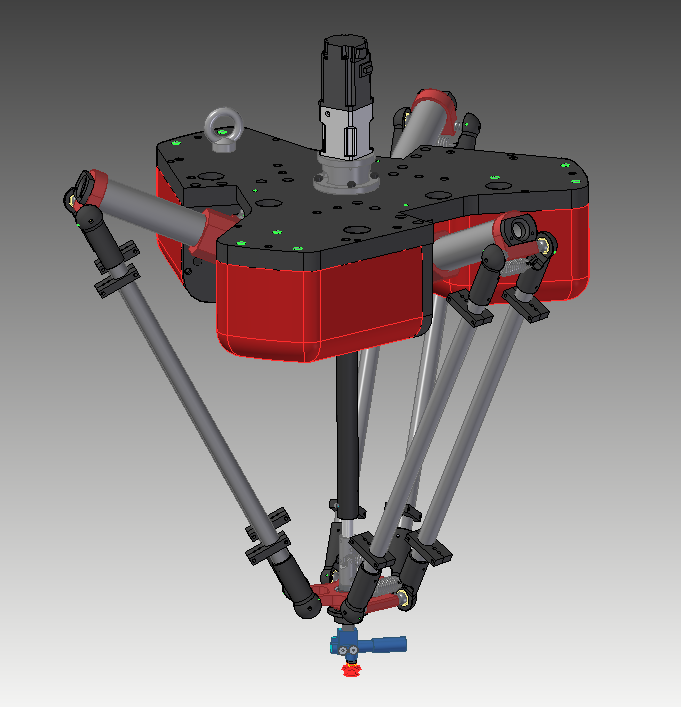
\includegraphics{./images/Deltacon_picture.png}}}\hspace{5pt}
\subfloat[Kinematics.]{%
\resizebox*{7cm}{!}{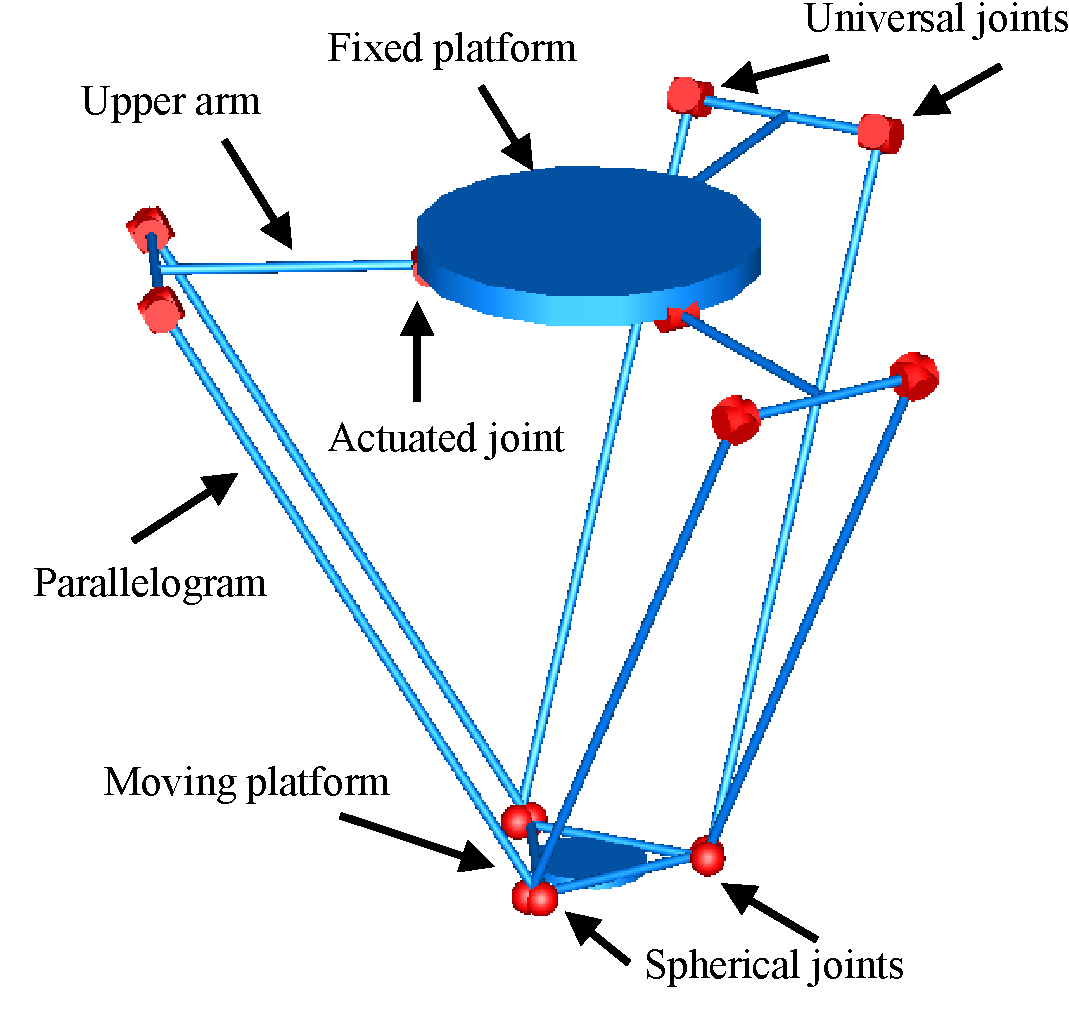
\includegraphics{./images/Deltacon_kinematics.pdf}}}
\caption{Delta robot.} \label{Fig:Delta_picture}
\end{figure}
The Delta robot here considered is the result of project developed in cooperation between \emph{Logicon} and \emph{Mitsubishi Electric Italia}. The servomotors and the relevant motion hardware and software were provided by Mitsubishi Electric Italia, while the mechanical components were purchased by third parties. Logicon was responsible for the assembly of the machine and for all other aspects related to the project, such as the design of the electrical cabinet, wiring, technical drawing and FEM analysis. Fig. \ref{Fig:Delta_picture}(a) shows a picture of the platform, while Fig. \ref{Fig:Delta_picture}(b) illustrates its kinematics.

The structure of the robot consists of three identical legs connecting a fixed base with a moving platform. Each leg is composed of an upper arm and a parallelogram structure; three actuated revolute joints connect the upper arms with the base and provide motion, while all other joints are spherical joints. However, the two upper spherical joints have been replaced by two universal joints, in order to avoid the long sides of the parallelogram to rotate along their axes.

\begin{figure}
\centering
\subfloat[Top level.]{%
\resizebox*{7.2cm}{!}{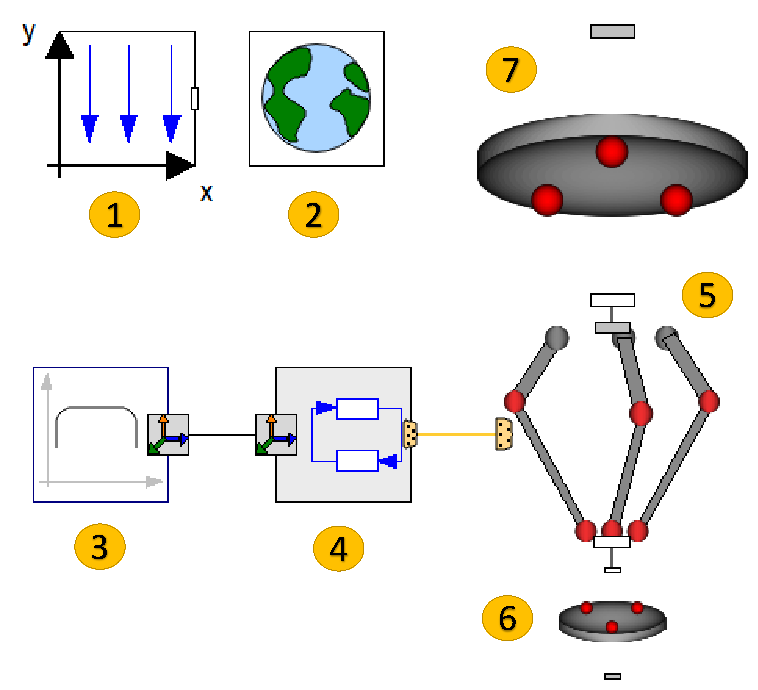
\includegraphics{./images/Delta_robot_Modelica_top_level.pdf}}}
\subfloat[Legs.]{%
\resizebox*{5.8cm}{!}{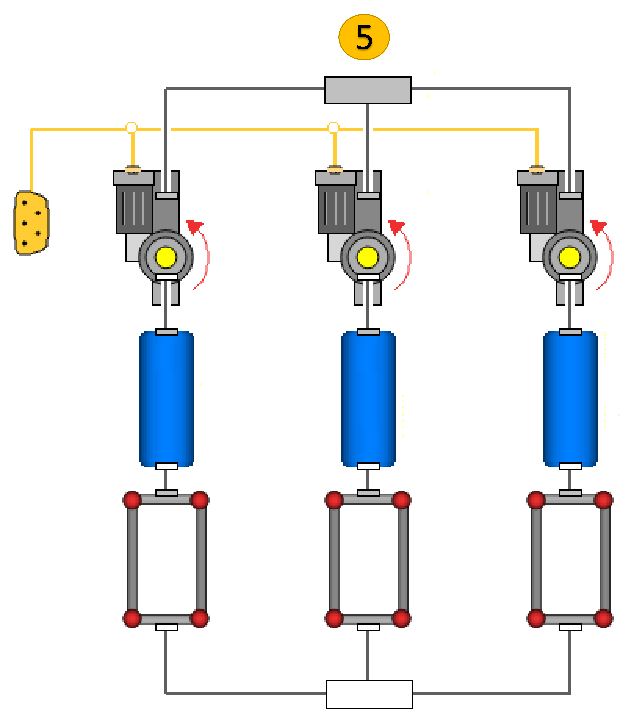
\includegraphics{./images/Delta_robot_Modelica_legs.pdf}}}
\caption{Delta robot: top level and legs models} \label{Fig:Delta_robot_Modelica_top_level}
\end{figure}
The top level Modelica model is shown in Fig. \ref{Fig:Delta_robot_Modelica_top_level}(a), it includes the world reference (1), the global parameters record (2), the motion planner (3), the motion controllers (4), the platform (6) and the base (7) models and the aggregate model of the legs (5), shown in Fig. \ref{Fig:Delta_robot_Modelica_top_level}(b).

The world reference model (1) defines the inertial reference frame and the gravity field (it must be always present when the \code{package MultiBody} is used \cite{dlr11987}), while the global parameters record (2) collects all the main parameters of the model to improve readability and modifiability.

The motion planner (3) defines the trajectory of the origin of the platform reference frame; so far linear, trapezoidal and cubic trajectories can be assigned, as well as the pick-and-place trajectory considered for validation.

The motion controller model (4) first implements the inverse kinematics, thus computing the reference signals for the controllers of the motor coordinates: 3 identical classical independent PID controllers have been implemented.

It must be noted that controllers are connected to servomotors through an \code{expandable connector}, denoted by the yellow cable connector. This (input/output) connector models the role of the communication bus on the real machine, collecting the control signals, thus the encoder measurements from the servomotors and the current setpoints from the controllers.

\begin{figure}
\centering
\subfloat[Actuator.]{%
\resizebox*{5cm}{!}{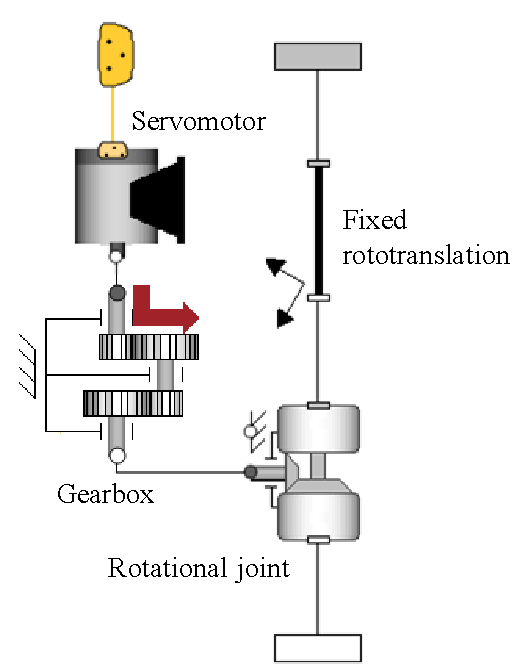
\includegraphics{./images/Delta_robot_Actuator.pdf}}}\hspace{5pt}
\subfloat[Parallelogram.]{%
\resizebox*{5cm}{!}{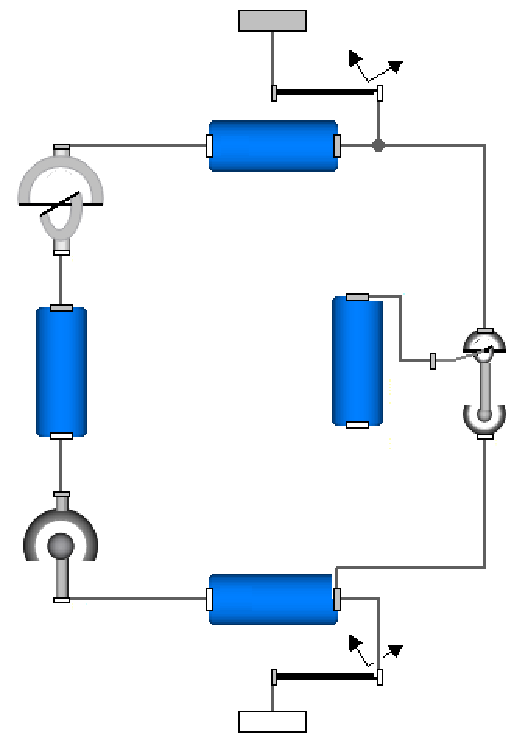
\includegraphics{./images/Delta_robot_Parallelogram.pdf}}}
\caption{Delta robot: leg model} \label{Fig:Delta_robot_Modelica_leg_model}
\end{figure}
The leg model is defined by the actuator model (Fig. \ref{Fig:Delta_robot_Modelica_leg_model}(a)) connected to the upper arm (rigid body), in turn rigidly connected to the upper short side of the parallelogram (Fig. \ref{Fig:Delta_robot_Modelica_leg_model}(b)).

The model of the electrical motor could have been easily included \cite{FMRBM2002} in the servomotor model, but this would have required the adoption of very short integration step sizes, needed to follow the electrical dynamics of the windings. Since in this work the focus is on the much slower mechanical dynamics, the whole current (torque) control loop has been approximated with a first order transfer function, modelling the torque control loop bandwidth.

The gearbox model has been taken directly from the Modelica standard library \cite{PSO20002}. In particular, the (lossy) gearbox model models the gear ratio and the losses of a standard gear box, including the stuck phases that may occur at zero speed, due to the friction in the gear teeth and/or in the bearings. The loss terms, efficiencies and friction torques, can be arbitrarily defined through lookup tables as functions of the absolute value of the input shaft speed and of the power flow direction.

\begin{figure}
\centering
\subfloat[Base.]{%
\resizebox*{4.5cm}{!}{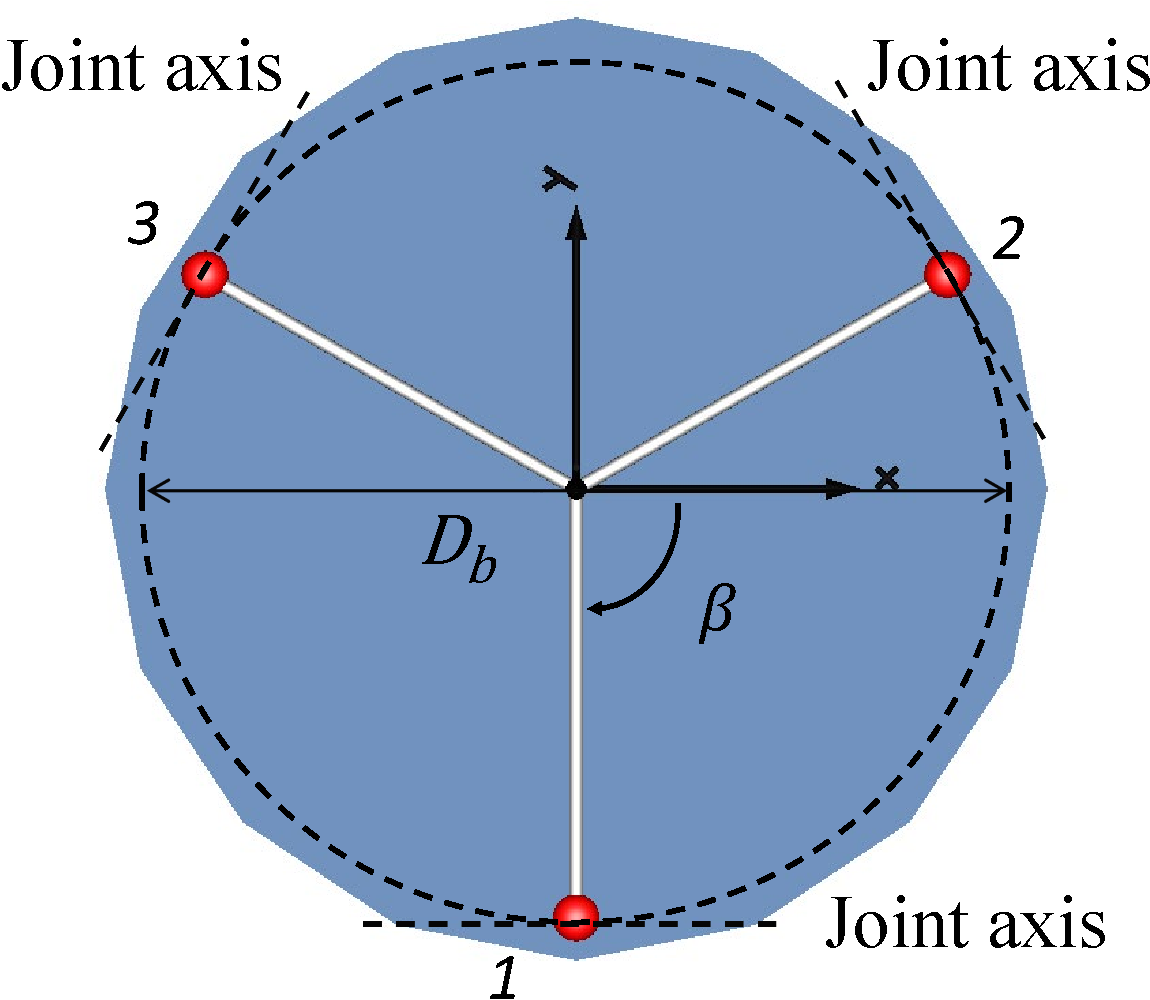
\includegraphics{./images/Deltacon_base.pdf}}}\hspace{1cm}
\subfloat[Platform.]{%
\resizebox*{3.8cm}{!}{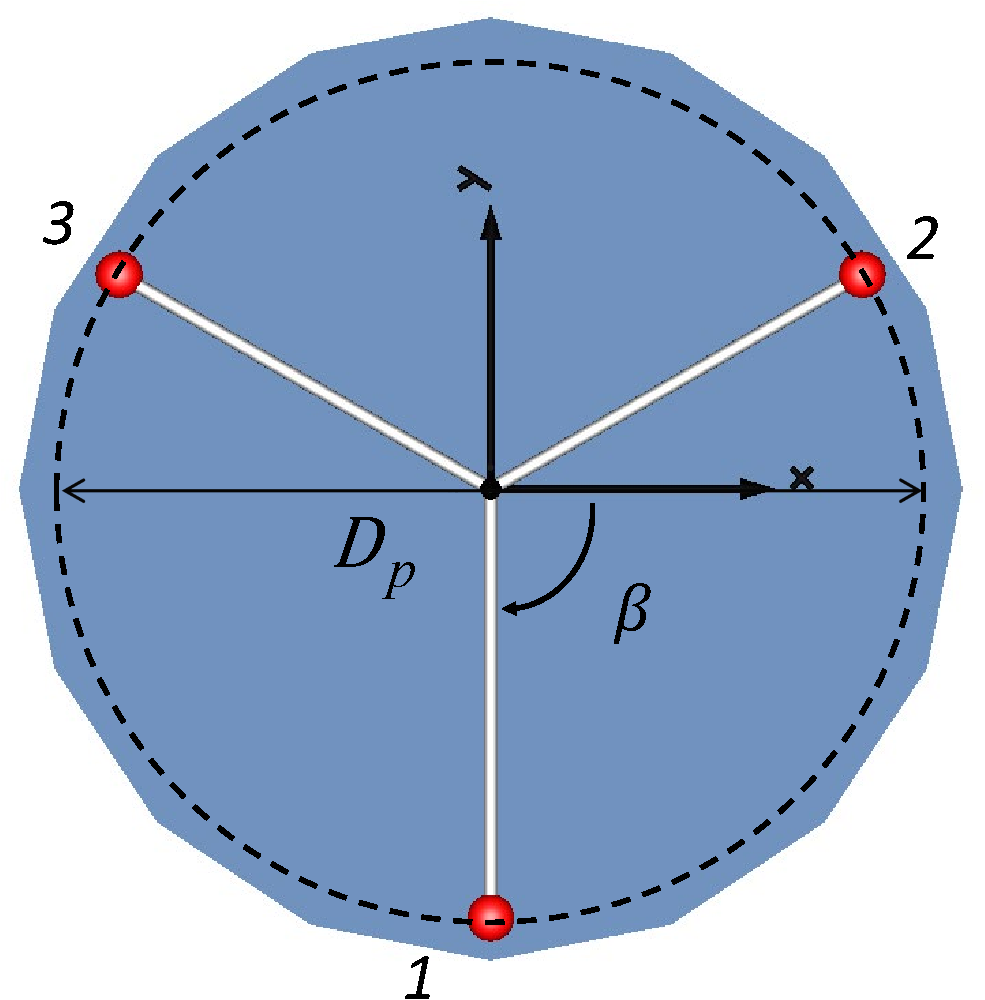
\includegraphics{./images/Deltacon_platform.pdf}}}
\caption{Deltacon base and platform.} \label{Fig:Deltacon_kinematics_parameters}
\end{figure}
The base (6) and the platform (7) can have different shapes and geometries, however, the kinematics is only defined by their attached reference frames, while dynamics is only defined by the inertial parameters of a single rigid body; in this case both base and platform have been modelled as discs (cylinders).

The upper arm rotational joints are attached to the base along a circumference of diameter $D_b$, displaced by 120$^\circ$, with the rotation axes tangent to the circumference (Fig. \ref{Fig:Deltacon_kinematics_parameters}(a)). The platform is attached to the lower sides of the parallelograms through frames placed along a circumference of diameter $D_p$, still displaced by 120$^\circ$ (Fig. \ref{Fig:Deltacon_kinematics_parameters}(b)).

It must be pointed out that the upper and lower connectors of the legs model in Fig. \ref{Fig:Delta_robot_Modelica_top_level}(b) are actually vector connectors. In other words, all the servomotors connectors and the connectors attached to the lower sides of the parallelograms are collected in a vector one, in turn connected to another vector connector of the base and platform. The base and platform models then define the correct geometrical displacements among the legs connectors through fixed rototranslation models.

\textcolor{blue}{
The model was built using library joints, which potentially introduce the state variables associated with the introduced degrees of freedom.
As a consequence of the closure of the kinematic chains, however, the degrees of freedom are only those associated with the actuators and, properly, the state variables of the model should be associated with the actual degrees of freedom only.
To implement this choice and guide the symbolic manipulation, the construct \code{StateSelect.always} was used for the variables of the actuators (position and speed) and \code{StateSelect.never} for the variables of all the other joints.
}

\textcolor{blue}{
Another problem concerns the initialization of the model, in particular the need to solve closed kinematic chains.
Also in this case it was decided to set the actuator variables using the \code{fixed = true} attribute, and then define the initial values of all the other variables as attempt values.
}

\textcolor{red}{
Validazione sperimentale.
\begin{itemize}
  \item Userei i dati della Simulazione 1, se fosse quella relativa al confronto fra animazione e video, metterei il link al video.
  \item Proverei ad imporre le coppie misurate e a fare il confronto fra le posizioni e le velocit\`{a} del modello e del robot
  \item Se non fosse un granch\`{e} metterei invece il confronto della tesi.
\end{itemize}
}

\section{Model of a Stewart platform}
\label{Sec:Stewart_platform_model}

\begin{figure}
\centering
\subfloat[Picture.]{%
\resizebox*{4cm}{!}{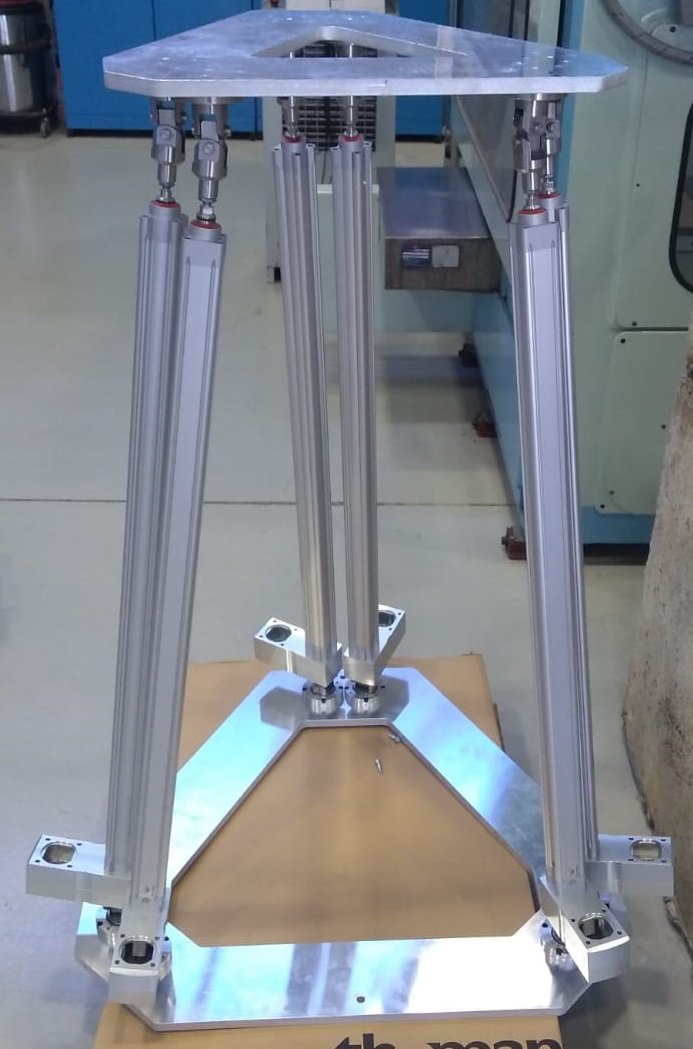
\includegraphics{./images/Stewart_photo.jpeg}}}\hspace{5pt}
\subfloat[Kinematics.]{%
\resizebox*{9cm}{!}{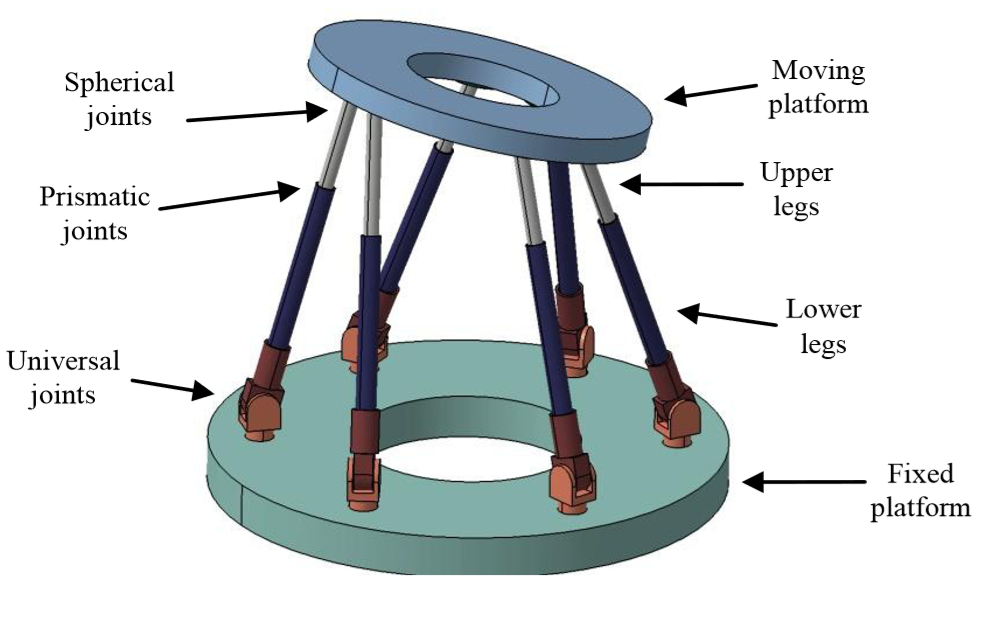
\includegraphics{./images/Stewart_kinematics.png}}}
\caption{Stewart platform.} \label{Fig:Stewart_platform_picture}
\end{figure}
The Stewart platform considered in this work has been designed for an innovative labeller for bottles of different size and dimension, Fig. \ref{Fig:Stewart_platform_picture}(a) shows a picture of the platform, while Fig. \ref{Fig:Stewart_platform_picture}(b) illustrates its kinematics.

It consists of a base and a platform, the former is usually fixed to the ground, while the latter can be positioned in space, in both position and orientation (6 d.o.f.), through 6 identical legs. Each leg is extendable through an electric cylinder, connected to the base through universal joints and to the moving platform through spherical joints. The electric cylinder is a mechanical linear drive unit with a piston rod, the driving component consists of an electrically actuated spindle converting the rotary motion of the motor into a linear motion of the piston rod.

\begin{figure}
\centering
\subfloat[Stewart platform: top level.]{%
\resizebox*{7cm}{!}{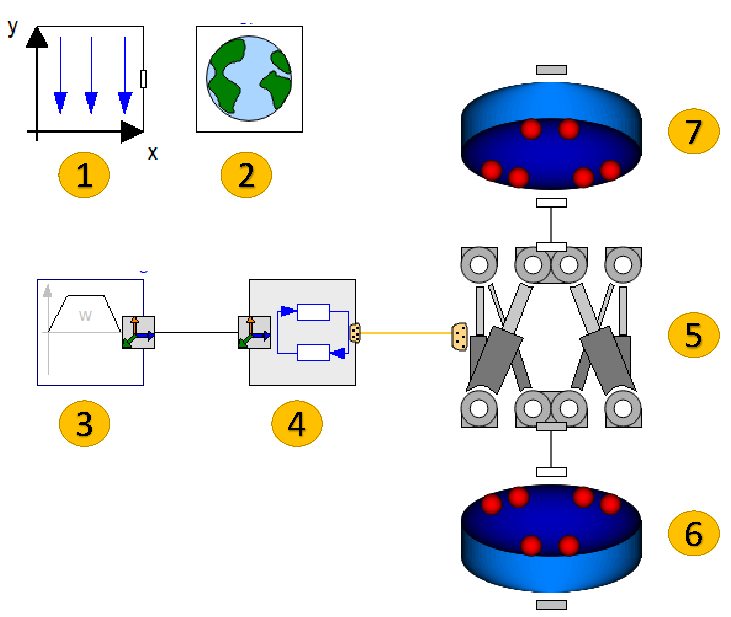
\includegraphics{./images/Stewart_platform_Modelica_top_level.pdf}}}
\subfloat[Stewart platform: legs.]{%
\resizebox*{5cm}{!}{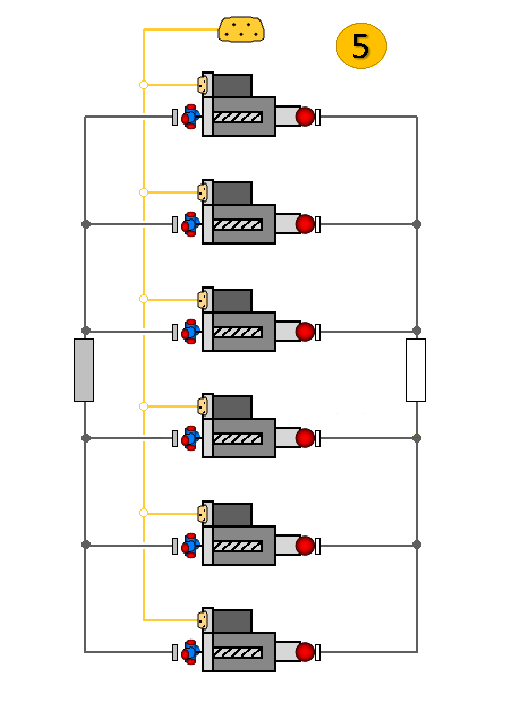
\includegraphics{./images/Stewart_platform_Modelica_legs.pdf}}}
\caption{Stewart platform: top level and legs models} \label{Fig:Stewart_platform_Modelica_top_level}
\end{figure}
The top level Modelica model is shown in Fig. \ref{Fig:Stewart_platform_Modelica_top_level}(a) and is very similar to the Delta robot top model, while the aggregate model of the legs (5) is shown in Fig. \ref{Fig:Stewart_platform_Modelica_top_level}(b).

In this case the motion planner (3) defines the trajectory of platform pose, in turn defined by the position of the origin of the platform reference frame and by the Euler angles relating the orientation of the platform frame with respect to the world frame; so far linear, trapezoidal and cubic trajectories can be assigned. Accordingly, 6 identical classical independent PID controllers have been implemented for the motion of the cylinders.

\begin{figure}
\centering
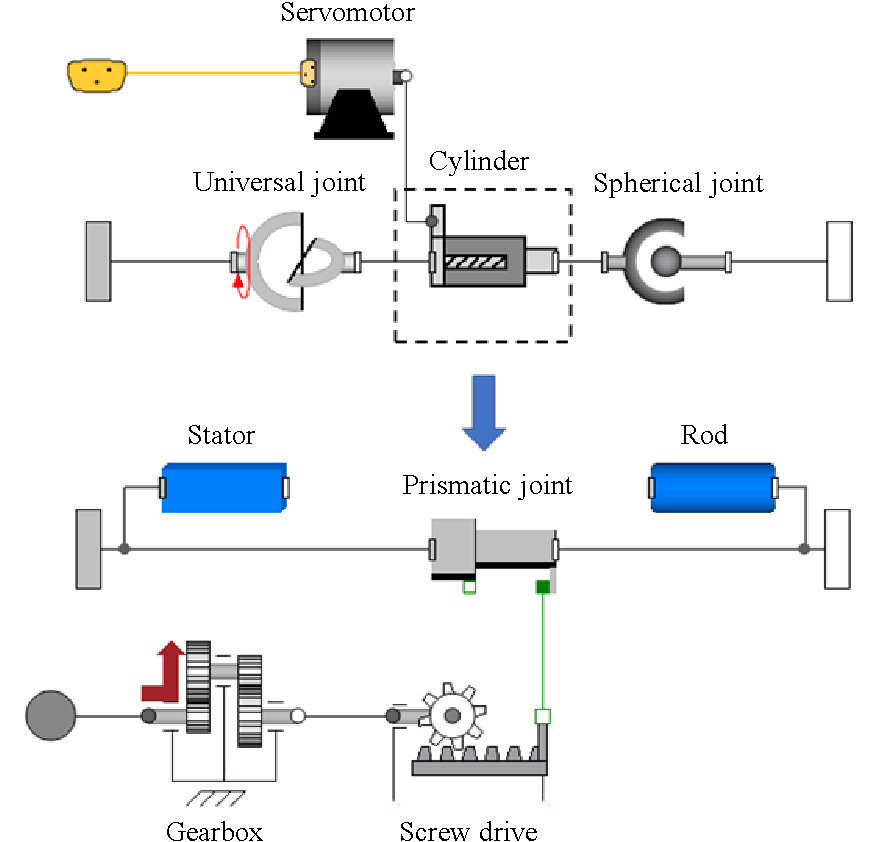
\includegraphics[width=0.65\columnwidth]{./images/Stewart_platform_Modelica_leg.pdf}
\caption{Stewart platform: leg model} \label{Fig:Stewart_platform_Modelica_leg}
\end{figure}
The leg model, whose hierarchy is shown in Fig. \ref{Fig:Stewart_platform_Modelica_leg}, is defined by the servomotor model connected to the cylinder model. In turn, the cylinder model is defined by the connection of two rigid bodies (stator and rod) through a prismatic joint, connected to the servomotor model through a gearbox model and a screw drive model. The Modelica standard library model of the ideal gear transforming rotational into translational motion has been slightly modified, in order to account for power losses, by simply defining two different transmission ratios for displacements and forces.
%namely the following equations have been implemented:
%\begin{eqnarray*}
%% \nonumber to remove numbering (before each equation)
%  &&\phi - \phi_0 = \rho_{\phi} (s - s_0) \\
%  &&\tau + \rho_{\tau} f = 0 \\
%  &&P_l = \tau \dot{\phi} \left(1 - \frac{1}{\rho_{\phi}\rho_{\tau}}\right)
%\end{eqnarray*}
%where $\phi$ is the nut angle and $\phi_0$ its reference value, $\rho_{\phi}$ and $\rho_{\tau}}$ are the transmission ratios for displacements and forces respectively,  for
%in the following Modelica model
%\begin{lstlisting}
%model RotationToTranslation
%    parameter Real rho_phi(final unit="rad/m", start=1);
%    parameter Real rho_tau(final unit="N.m/N", start=1);
%    parameter SI.Angle phi0=0;
%    parameter SI.Position s0=0;
%    SI.AngularVelocity w;
%    SI.Power Pl;
%    Modelica.Mechanics.Rotational.Interfaces.Flange_a flangeR;
%    Modelica.Mechanics.Translational.Interfaces.Flange_b flangeT;
%equation
%    (flangeR.phi - phi0) = rho_phi*(flangeT.s - s0);
%    0 = flangeR.tau + rho_tau*flangeT.f;
%    w = der(flangeR.phi);
%    Pl = flangeR.tau*w*(1 - 1/(rho_tau*rho_phi));
%end RotationToTranslation;
%\end{lstlisting}

\begin{figure}
\centering
\subfloat[Base.]{%
\resizebox*{5cm}{!}{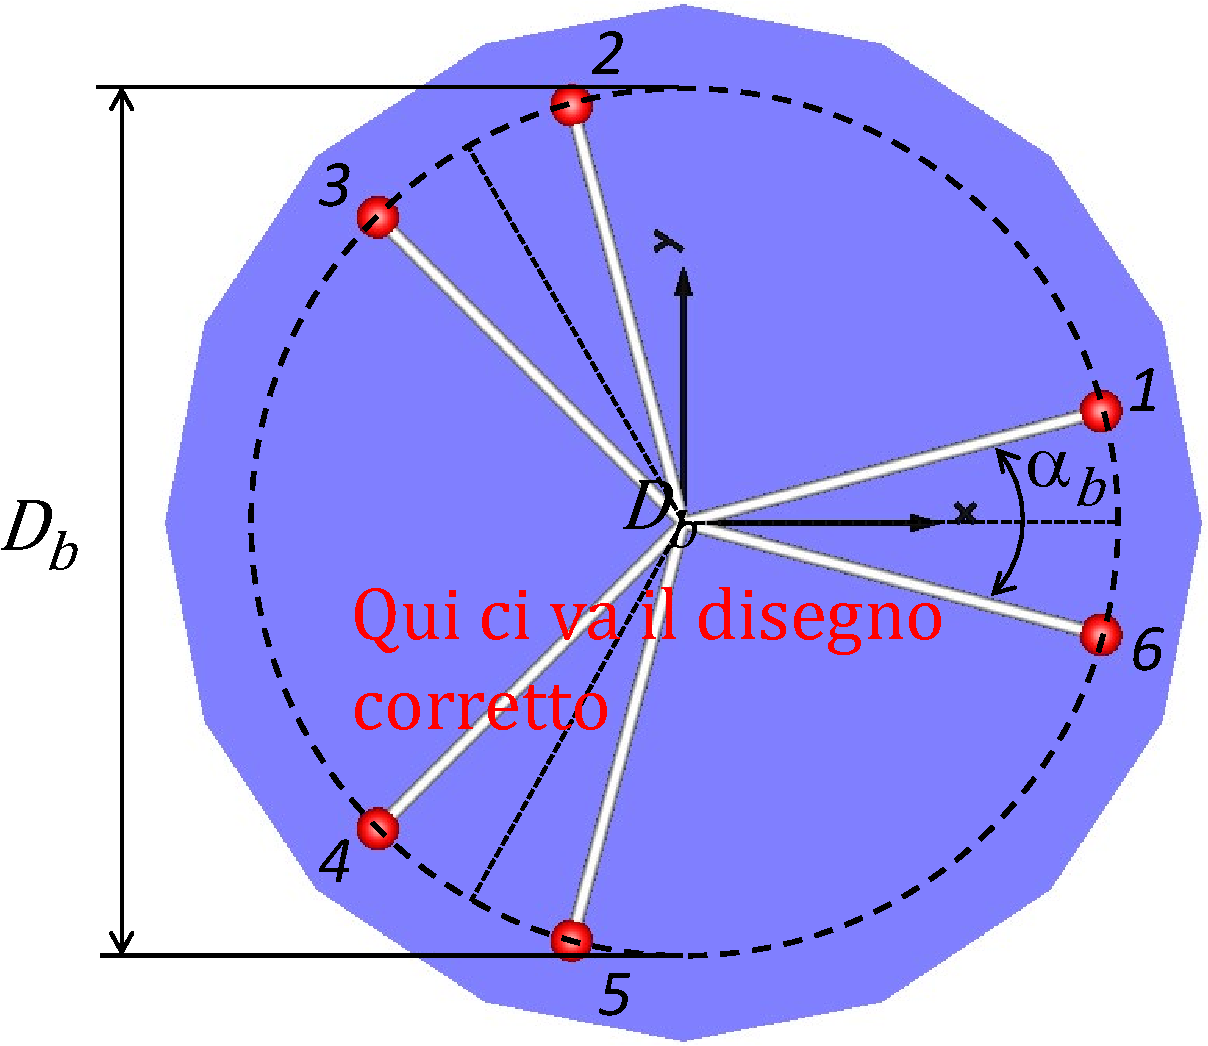
\includegraphics{./images/Stewart_base.pdf}}}\hspace{1cm}
\subfloat[Platform.]{%
\resizebox*{5cm}{!}{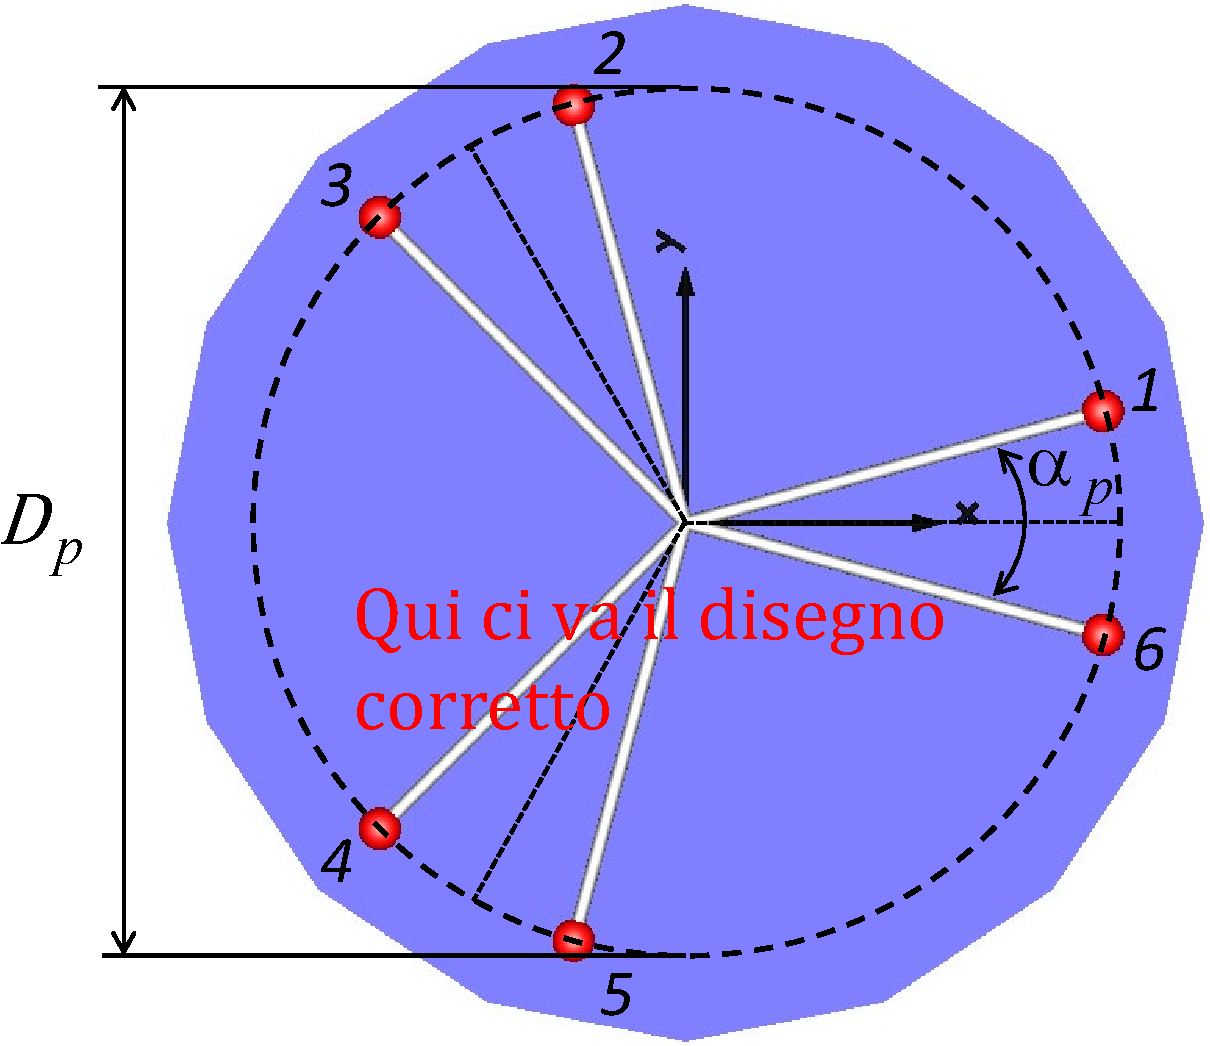
\includegraphics{./images/Stewart_platform.pdf}}}
\caption{Stewart platform kinematics parameters.} \label{Fig:Stewart_platform_kinematics_parameters}
\end{figure}
The positions of the joints on the base and platform are placed on a circumference, of diameters $D_b$ and $D_p$, in couples displaced by 120$^\circ$, with $\alpha_b$, $\alpha_p$ being the angular displacements between the positions of each couple (Fig. \ref{Fig:Stewart_platform_kinematics_parameters}). The right and left connectors of the legs model in Fig. \ref{Fig:Stewart_platform_Modelica_top_level}(b) are again vector connectors, connected to other vector connectors on the base and platform.

%The models of base (6) and platform (7) are shown in Fig. \ref{Fig:Stewart_platform_base_and_platform}
%\begin{figure}
%\centering
%\subfloat[Base model.]{%
%\resizebox*{5cm}{!}{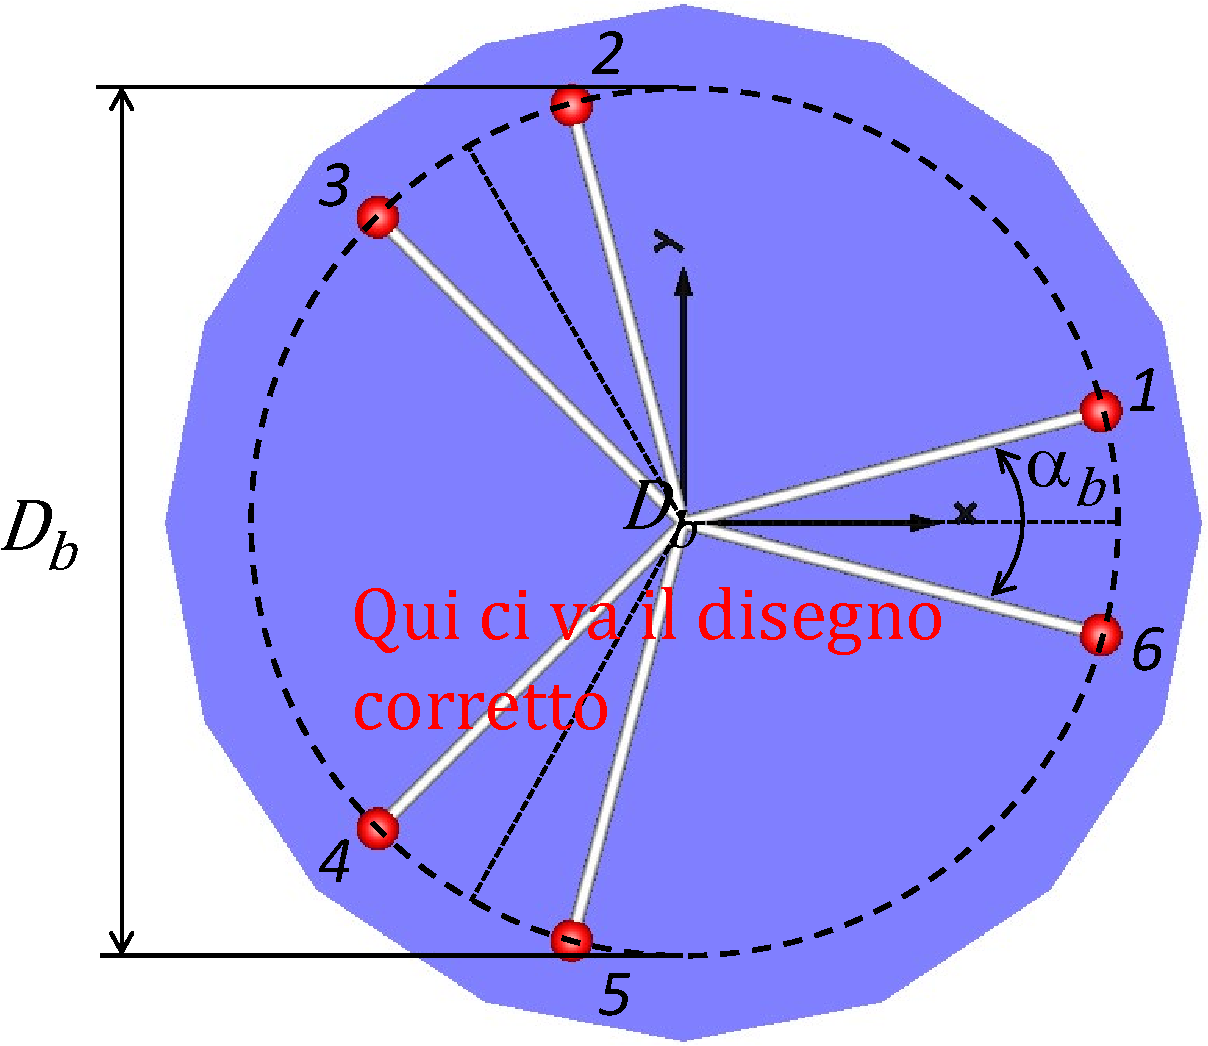
\includegraphics{./images/Stewart_base.pdf}}}\hspace{1cm}
%\subfloat[Platform model.]{%
%\resizebox*{5cm}{!}{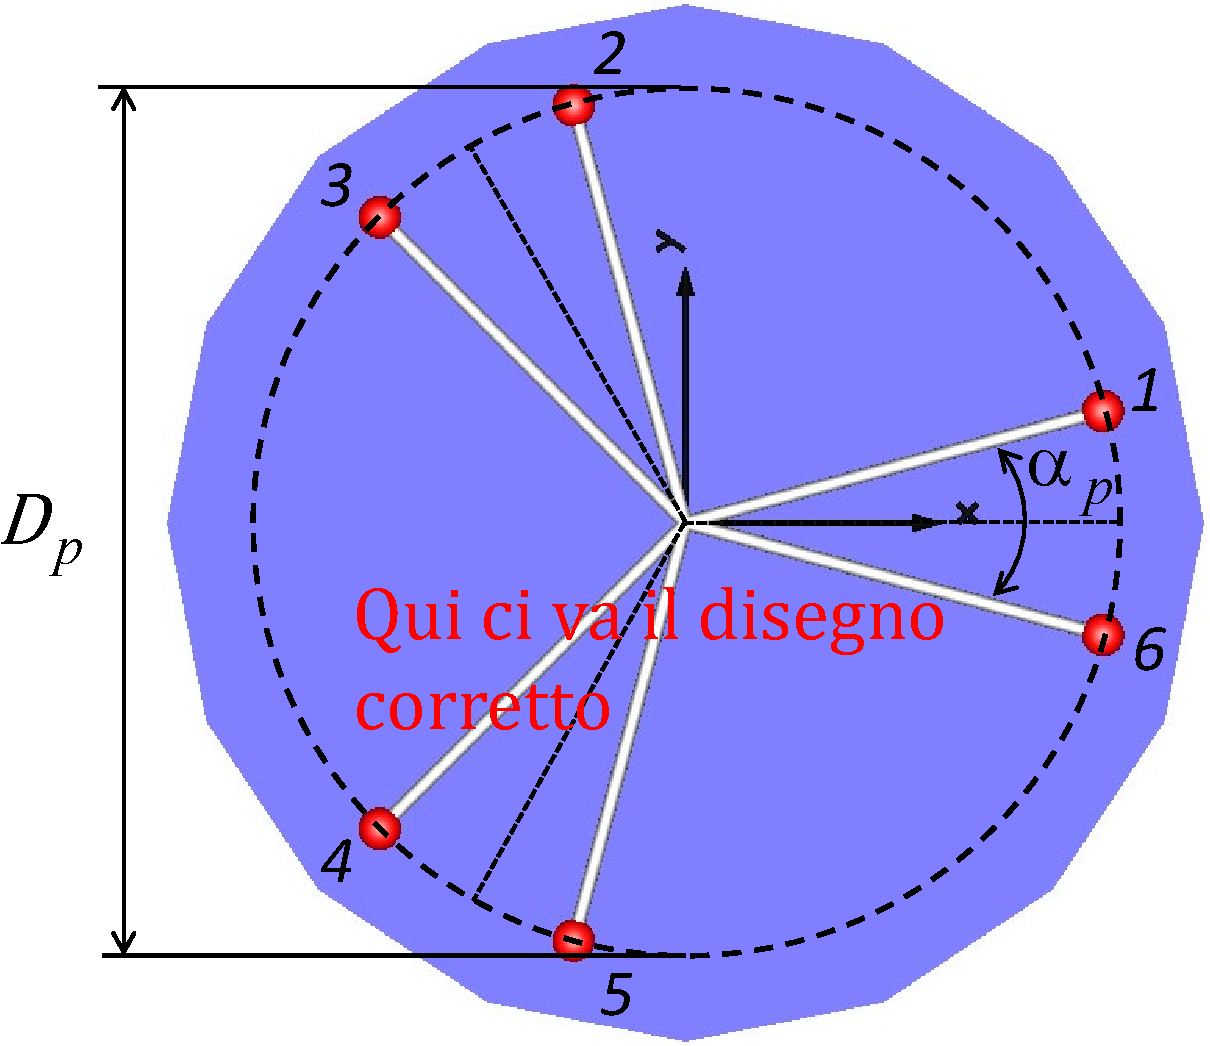
\includegraphics{./images/Stewart_platform.pdf}}}
%\caption{Stewart platform base and platform models.} \label{Fig:Stewart_platform_base_and_platform}
%\end{figure}

\section{Computation of the inverse dynamics for the Stewart platform}
\label{Sec:Inverse_dynamics}

\textcolor{red}{
\begin{enumerate}
 \item Si considera il modello controllato della piattaforma di Stewart, le cui uscite, posizioni, velocità ed accelerazioni dell'end effector saranno gli ingressi del modello inverso.
  \item Si crea il modello inverso e si verifica che le coppie calcolate dal modello diretto e inverso siano identiche.
  \item Si crea l'FMU del modello inverso.
  \item Si verifica che le uscite del modello inverso OpenModelica e FMU siano identiche.
  \item Si incapsula l’FMU in un file C per verificare i tempi di calcolo.
\end{enumerate}
}

\section{Conclusion}
\label{Sec:Conclusion}

Conclusion.

\bibliographystyle{tfq}
\bibliography{OOParallel}

%\appendix
%
%\section{Appendice}
%
%Appendix.

\end{document}
